\documentclass[11pt]{article}
\usepackage{geometry,marginnote} % Pour passer au format A4
\geometry{hmargin=1cm, vmargin=1.5cm} % 

% Page et encodage
\usepackage[T1]{fontenc} % Use 8-bit encoding that has 256 glyphs
\usepackage[english,french]{babel} % Français et anglais
\usepackage[utf8]{inputenc} 

\usepackage{lmodern}
\usepackage[np]{numprint}
\setlength\parindent{0pt}

% Graphiques
\usepackage{graphicx,float,grffile}
\usepackage{tikz,pst-eucl,pst-plot,pstricks,pst-node,pstricks-add,pst-fun,pgfplots} 

% Maths et divers
\usepackage{amsmath,amsfonts,amssymb,amsthm,verbatim,scratch3}
\usepackage{multicol,enumitem,url,eurosym,gensymb,tabularx}

\DeclareUnicodeCharacter{20AC}{\euro}



% Sections
\usepackage{sectsty} % Allows customizing section commands
\allsectionsfont{\centering \normalfont\scshape}

% Tête et pied de page
\usepackage{fancyhdr} \pagestyle{fancy} \fancyhead{} \fancyfoot{}

%\fancyfoot[L]{Collège Faubert}
%\fancyfoot[C]{\thepage / 6}
%\fancyfoot[R]{Série Générale}

\renewcommand{\headrulewidth}{0pt} % Remove header underlines
%\renewcommand{\footrulewidth}{0pt} % Remove footer underlines

\newcommand{\horrule}[1]{\rule{\linewidth}{#1}} % Create horizontal rule command with 1 argument of height

\newcommand{\Pointilles}[1][3]{%
  \multido{}{#1}{\makebox[\linewidth]{\dotfill}\\[\parskip]
}}

\newtheorem{Definition}{Définition}

\usepackage{siunitx}
\sisetup{
    detect-all,
    output-decimal-marker={,},
    group-minimum-digits = 3,
    group-separator={~},
    number-unit-separator={~},
    inter-unit-product={~}
}

\setlength{\columnseprule}{1pt}


\begin{document}

\textbf{Nom, Prénom :} \hspace{8cm} \textbf{Classe :} \hspace{3cm} \textbf{Date :}\\

\begin{center}
  \textit{On ne craint que ce que l'on ne connaît pas.} - \textbf{Marie Curie}
\end{center}


\textbf{ex1 - Calculer}

\begin{multicols}{3} \begin{itemize}[label={$\bullet$}]
  \item $\dfrac{5}{21} + \dfrac{5}{21} =$ \dotfill
  \item $\dfrac{14}{15} + \dfrac{5}{15} - \dfrac{7}{15}  =$ \dotfill
  \item $\dfrac{32}{45}  + \dfrac{8}{45} - \dfrac{10}{45}  =$ \dotfill
\end{itemize} \end{multicols}

\textbf{ex2 - Calculer}

\begin{multicols}{3} \begin{itemize}[label={$\bullet$}]
  \item $5 \times \dfrac{1}{3} =$ \dotfill
  \item $8 \times \dfrac{2}{7} =$ \dotfill
  \item $4 \times \dfrac{1}{45}  + 10 \times \dfrac{3}{45} =$ \dotfill
\end{itemize} \end{multicols}


\textbf{ex3 - Calculer}

\begin{multicols}{3} \begin{itemize}[label={$\bullet$}]
  \item $\dfrac{14}{14} =$ \dotfill
  \item $\dfrac{88}{8} =$ \dotfill
  \item $\dfrac{45}{5} =$ \dotfill
\end{itemize} \end{multicols}

\textbf{ex4 - Calculer}

\begin{multicols}{2} \begin{itemize}[label={$\bullet$}]
  \item $1 + \dfrac{4}{10} =$ \dotfill
  \item $4 + \dfrac{5}{8} =$ \dotfill
  \item $11 + \dfrac{17}{7} =$ \dotfill
  \item $5 + \dfrac{16}{12} =$ \dotfill
\end{itemize} \end{multicols}

\textbf{ex5 - Représenter}

\begin{figure}[H]
  \centering
  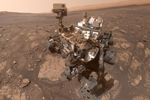
\includegraphics[width=0.7\linewidth]{6x1-fractions/ex5.pdf}
\end{figure}


\textbf{ex6 - Représenter}

\begin{figure}[H]
  \centering
  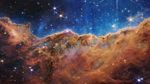
\includegraphics[width=0.7\linewidth]{6x1-fractions/ex6.pdf}
\end{figure}


\textbf{ex7 - Démontrer}

\begin{multicols}{2}
  \begin{eqnarray*}
    \dfrac{41}{5} &=& \\
                  &=& \\
                  &=& 8 + \dfrac{1}{5}
  \end{eqnarray*} \columnbreak
  
  \begin{eqnarray*}
    \dfrac{79}{11} &=& \\
                  &=& \\
                  &=& 
  \end{eqnarray*}

\end{multicols}

\end{document}